\section{Step Obstacles}
Some non-lethal obstacles are defined by a flat step cost, such as the interaction areas of \citet{fraichard:anthronav} or the perimeter of the parking lot in \citet{likhachev:costmaps}. In this trivial case, the marginal cost is
\begin{equation}
   \displaystyle
   f(x, y) = \left\{
     \begin{array}{lr}
       A & : (x,y) \in Q\\
       0 & : (x,y) \notin Q
     \end{array}
   \right.
\end{equation}
Each step traversing the obstacle costs a premium $A$. 

\begin{figure}[!t]
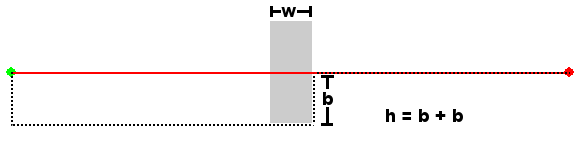
\includegraphics[width=\columnwidth]{graphix/Constant.png}
\caption{Two Paths with a Constant Non-lethal obstacle}
\label{fig:constant}
\end{figure}

We will plan a path from $(n, 0)$ to $(-n, 0)$, computing the cost by summing the baseline cost-per-step $P$ and the marginal cost-per-step $f$ over each step.

\begin{equation}
C(p) = \sum\limits_p P + f(x, y)
\end{equation}

For a rectangular step obstacle placed at the origin with dimensions $w\times h$, there are essentially two feasible paths, illustrated in Figure \ref{fig:constant}. The direct path costs
\begin{equation}
C(p_1) = 2nP + wA
\end{equation}

The shortest path around the obstacle costs

\begin{equation}
C(p_2) = (2n + h)P.
\end{equation}

The direct path is cheaper when the aspect ratio of the obstacle  is greater than the fractional cost penalty:

\begin{equation}
\frac{h}{w} > \frac{A}{P}.
\end{equation}

This result is intuitive. If an obstacle is thin or insubstantial, walk through it.




